
\documentclass[journal]{IEEEtran}
\usepackage{cite}
\usepackage[utf8]{inputenc}
\usepackage{caption}
\usepackage{url}
\usepackage{amssymb}
\usepackage{amsmath}
\usepackage{algorithm}
\usepackage{graphicx}
\graphicspath{ {images/} }

% correct bad hyphenation here
\hyphenation{op-tical net-works semi-conduc-tor}


\begin{document}


% paper title
\title{Review of procedural content generation methods and applications}

% author names and IEEE memberships
\author{
Bojan Lovrovic\\
\textit{Faculty of Electrical Engineering and Computing}\\
\textit{University of Zagreb}\\
\textit{Zagreb, Hrvatska}

\thanks{}
}

% make the title area
\maketitle

\section{Uvod}
\IEEEPARstart{P}{}rocedural content generation (PCG) is the programmatic generation of content using a random or pseudo-random process that results in an unpredictable range of possible assets, whether it be geometry, textures, sounds or even narratives. It can also be combined with other different methods such as machine learning. This paper will present an introduction to random number generation, then move to varying methods used in PCG and their application in virtual worlds such as computer generated imagery, video games, virtual realities, simulations and so forth.

\section{Pregled područja}
\subsection{Broad classification}
There are two competing methodologies in procedural content generation. The first approach creates a physical model of the environment and the process that creates the generated object, then simply runs the simulation, and the results should emerge as they do in nature. Examples of such algorithms and simulations are, among others, dynamic weather, fire propagation, fluid dynamics, genetic algorithm and rain drop algorithm.
\par
Ad hoc\footnote{A non-generalizable solution designed for a specific problem or task.} type of algorithms are the second approach, in which we observe the end results of this process and then attempt to directly reproduce those results. Examples are perlin noise, simplex noise and voronoi diagram generation.
\subsection{Random number generators}
The most basic and fundamental part of every PCG is its pseudorandom number generator (PRNG). The approach is not truly random as it produces the same series of numbers for a given algorithm and initialization value known as \textit{seed}. Memory and time complexity play a crucial role in every algorithm assessment and PRNG algorithms do not differ in this regard. There is, however, one parameter more important as it directly affects the variety of generated results. This parameter is known as \textit{period} and it represents the maximum, over all starting states, of the length of the repetition-free prefix of the sequence. If the PRNG uses \textit{n} bits to represent the current state it is in, then the period of a series cannot be longer than $2^{n}$ results, and may be much shorter. The randomness of the results can also be checked with various tests, among which is a most widely used battery of tests called the \textit{diehard tests} \cite{diehard}.
\par
Of historical importance is the algorithm called linear congruential generator. The transition from state to state is given by the equation \ref{eq:LCG}.
\begin{gather}
\label{eq:LCG}
x_{n+1}=(a \cdot{x_n} + c)\mod{m}
\end{gather}
Where \textit{x\textsubscript{n}} is the current sate of the generator. The period of a LCG is at most m, and for some choices of factor a much less than that. Main advantage of this algorithm is it's speed but it still shouldn't be used in applications where high quality randomness is critical because of the serial correlation between the generated numbers.\par
Mersenne Twister is the most widely used and is first PRNG provide fast generation of high-quality pseudorandom integers. The most commonly used version is based on the Mersenne prime number\footnote{The Mersenne twister derives it's name from the fact that it's period is equal to the one of the Mersenne prime numbers. More can be found in \cite{mersennePrime}.} $2^{19937}-1$ which is also commonly the period of the sequence. The algorithm comes in two versions, 32-bit and 64-bit generated number size. Its main disadvantage is the size of the current state\footnote{There is a proposed version to address this issue. The tiny version, TinyMT, uses just 127 bits of state space.}, which can take up to  2.5 KiB. Other than that, it is considered somewhat slow by today's standards. The advantage besides a very long period is its ability to pass the \cite{diehard} tests for statistical randomness which makes it a good candidate for Monte Carlo methods.\footnote{a broad class of computational algorithms that rely on repeated random sampling to obtain numerical results. More in \cite{monteCarlo}}\par
Presented algorithms generate uniformly distributed series of numbers, but sometimes this does not suffice. Perfect example is trying to generate something that follows a Gaussian normal distribution like most occurrences in nature do. To tackle this problem, many different solutions to different distributions have been devised, but in this paper focus will solely be on the approaches for normal distribution. Three most widely used are the Box–Muller transform, which is the least efficient, Marsaglia polar method and the Ziggurat algorithm, the most efficient one. All three base their results on the input which is presumed to be an uniformly distributed series of numbers.
\par
The problem with pseudorandom generators is it's predictable nature. This is not so important in content generation but for applications such as encryption it can have devastating effects. Therefore algorithms such as \cite{twoSourceRandomNumGenerator} have been devised to create truly random number generators.
\subsection{Height map generators}\label{subsecHeightmap}
A method in PCG that is undoubtedly one of the most popular and widely used is terrain generation. This method belongs to the set of ad hoc approaches. In comparison to the amount of time it takes for the designer to produce the same results, terrain generators are fairly quick, and with the help of GPGPU\footnote{General-purpose computing on graphics processing units.} they are ostensibly instant. Perlin noise, named after it's author Ken Perlin, is the usual way of generating height maps.\par
The common procedure for Perlin noise texture generator, as described \cite{gpugems2} (chapter 26.), is to initialize a two dimensional array of two dimensional \textit{gradient vectors}, which are just random unit vectors. A scalar value, which in end represents the height of the heigh map, is calculated by taking the dot product between the gradient and the fractional position within the noise space. Each pixel is in a grid and therefore has four of this scalar values. In two dimensional case, bilinear interpolation can be used, although, bicubic interpolation is recommended to compute the final scalar value for a given pixel. The results of this can be seen in figure \ref{fig:gradientvectors}.\par
\begin{figure}[H]
	\centering
	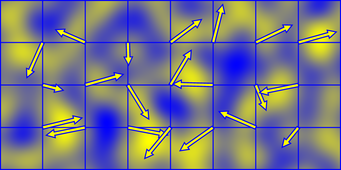
\includegraphics[width=.8\linewidth]{gradientField.png}
	\captionof{figure}{Grid with gradient vectors and resulting noise.}
	\label{fig:gradientvectors}
\end{figure}
This procedure, then, needs to be applied several times in a way fractals are computed. The same terminology is used, so \textit{octaves} is a number from $\mathbb{N}$ that represents how many times computed texture is pixel-wise summed with itself. Each summation is done with the result of the previous and the downscaled original. \textit{Lacunarity} has to do with the size distribution of the holes. Roughly speaking, if a height map has large gaps or holes, it has high lacunarity; on the other hand, if a height map is almost translationally invariant, it has low lacunarity. Often used when describing fractals is the \textit{basis function} and that would be, in our case, the dot product described previously. The height map derived from this method is shown in figure \ref{fig:perlinNoise}.\par
\begin{figure}[H]
	\centering
	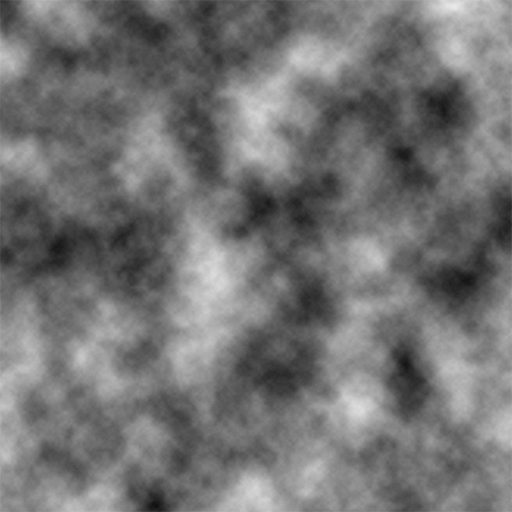
\includegraphics[width=.6\linewidth]{perlinNoise.png}
	\captionof{figure}{Perlin noise with a few octaves.}
	\label{fig:perlinNoise}
\end{figure}
Popular improvement is called \textit{Ridged multifractal} which uses the basis function same as typical Perlin noise generator but in composition with the function given in equation \ref{eq:ridgedFunc}.
\begin{gather}
\label{eq:ridgedFunc}
f(x)=\begin{cases}
2x & \text{ if } x < \frac{1}{2} \\ 
2(1-x) & \text{ if } x \geq \frac{1}{2}
\end{cases}
\end{gather}
When trying to generate occurrences in nature, this is usually combined with the typical Perlin noise to achieve more visually believable results.

\section{Implementacija}
Implementacija se temelji na \cite{giraffe}.

When talking about memory space reduction with PCG, the video game \textit{.kkrieger} is a good example of what can be achieved by generating assets only before use. The game requires only 97 kilobytes of disk space. If stored conventionally, it would require around 300 megabytes, according to developers.
\par
Another example is the upcoming video game called \textit{No Man's Sky} which should feature up to $2^{32}$ fully explorable procedurally generated worlds. Said worlds would include it's own specific flora and fauna, as well as unique terrain per world (see figure \ref{fig:nomansky}), meaning each world would use significant amount of memory. It is obvious that this would be impossible to store on computer memory as a whole and therefore PCG imposes itself as the only solution. Although the overall quality of the content is still questioned, the project has attracted a lot of attention.
\begin{figure}[H]
	\centering
	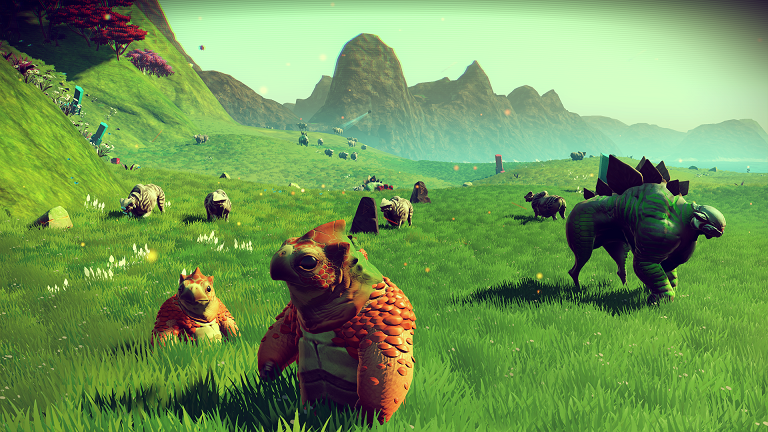
\includegraphics[width=.8\linewidth]{NoMansSky.png}
	\captionof{figure}{PCG from the video game No Man's Sky.}
	\label{fig:nomansky}
\end{figure}
\par
The greatest downside of using PCG as a space requirement reduction method is the need for generating data instead of loading it directly from storage, which is in most cases slower.

\section{PCG used to increase productivity}
One of the most widely used applications of PCG is to remove workload from designers and artists on projects that require creative type of work. This ranges from generating random noise in image editor, all the way to creating entire sequences of animation in a story driven dialogue.
\par
\textit{Witcher 3} is a video game that is an example of the latter. It enables designers to generate animation based on the information about the actors, some cinematic instructions and the extracted information from voice audio data files. After generation, the designers step in to verify the results and modify if it's required. The downside of such approach is that it required software engineers to create the program for this purpose and it still needed designer's touch after it's been used. However, considering the size of the video game and the amount of animations that were needed, it turned out to be a good investment to relay on PCG, developers claim.
\par
Another interesting example of this PCG application is a project called \textit{Mark Maker}\footnote{Their website: http://emblemmatic.org/markmaker/} that creates logos for companies based on their name. What makes it more interesting is the fact that it uses machine learning to filter the results, after a few steps, that fit the user's taste the most.

\section{Simple example of PCG}
Example presented here is a simple space nebulae rendering. All the assets are generated on the GPU using a slightly modified versions of algorithms from subsection \ref{subsecHeightmap}.
\par
First a three-dimensional texture is created combining simple Perlin noise and a Ridged multifractal. This texture has dimension of 256 textels in it's width, depth and height which resulted in total memory of 32 megabytes (2 bytes were used per textel). Additionally a function was used to fade out the intensity of textels towards the edges of the texture in order to prevent the impression of nebulae being unnaturally cut in space.\par
\begin{figure}[H]
	\centering
	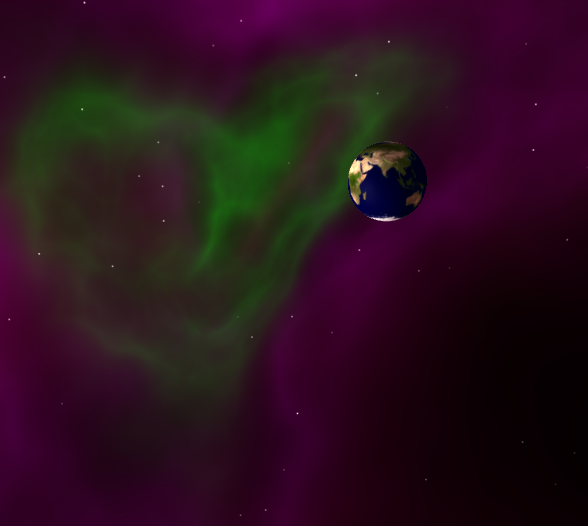
\includegraphics[width=.6\linewidth]{nebulae.png}
	\captionof{figure}{Scene of the generated nebulae with a planet.}
	\label{fig:nebulaescene}
\end{figure}
The texture is then used in a ray caster algorithm. Rays are projected from camera position towards each pixel in pixel shader program\footnote{Pixel shader program is executed on the GPU for each pixel that needs to be drawn for a given geometry. In this case the geometry is a full screen quad (a polygon that covers entire viewport).}. Each of those rays samples the texture in about fifty steps per ray and sums the sampled intensities for each pixel. The samples are not gathered along the entire ray because that would cause too many useless samples outside of the nebula space. Rather than that, intersection points between the ray and the incircle of the nebula texture are found (algorithm from \cite{christer}). Those two points are used as a ray's beginning and end, which results in every sampling step being useful.
\par
A function $f:\mathbb{R}\rightarrow\mathbb{R}^{3}$ is used to extract color from intensity values. This function is implemented as a one dimensional texture sampler. The said texture contains entire hue the nebula will be colored in. The end product can be seen in figure \ref{fig:nebulaescene}.

\section{Conclusion}
Although PCG is present for decades, it is still an approach being researched and with it's use rising. Increases in hardware capabilities also have a positive effect on this trend. On the other hand, there is a popular belief that PCG can never produce content as good as the artists or designers can. This is definitely true with today's hardware and software capabilities, so the question that poses itself is, where to draw the line. To what point should content be generated and then left out to professionals to do the rest. The approach of no Man's Sky, where almost everything is procedurally generated, seems too excessive, yet on the contrast, generating random noise in image editor pixel by pixel would be even worse. Whenever the line might be, it will surely move in avail of PCG and we are yet to see much more surprises from this field.

% Can use something like this to put references on a page
% by themselves when using endfloat and the captionsoff option.
\ifCLASSOPTIONcaptionsoff
  \newpage
\fi

\bibliographystyle{plain}
\bibliography{references}

\end{document}


